\documentclass[12pt]{article}
\usepackage{lecture}
\usepackage{graphics}
\usepackage{epstopdf}
\usepackage{html}
\usepackage{url}

\newcommand{\copyrightYears}{2001-2021}

\title{Introduction to molecular population genetics}

\begin{document}

\maketitle

\thispagestyle{first}

\section*{Introduction}

The study of evolutionary biology is commonly divided into two
components: study of the {\it processes\/} by which evolutionary
change occurs and study of the {\it patterns\/} produced by those
processes. By ``pattern'' we mean primarily the pattern of
phylogenetic relationships among species or genes.\footnote{In certain
  cases it may make sense to talk about a phylogeny of populations
  within species, but in many cases it doesn't. We'll discuss this
  further when we get to phylogeography in a couple of weeks.} Studies
of evolutionary processes often don't often devote too much attention
to evolutionary patterns, except insofar as it is often necessary to
take account of evolutionary history in determining whether or not a
particular feature is an adaptation. Similarly, studies of
evolutionary pattern sometimes try not to use any knowledge of
evolutionary processes to improve their guesses about phylogenetic
relationships, because the relationship between process and pattern
can be tenuous.\footnote{This approach is much less common than it
  used to be. In the ``old days'' (meaning when I was a young
  assistant professor), we had vigorous debates about whether or not
  it was reasonable to incorporate some knowledge of evolutionary
  processes into the methods we use for inferring evolutionary
  patterns. Now it's pretty much taken for granted that we should. One
  way of justifying a strict parsimony approach to cladistics,
  however, is by arguing (a) that by minimizing character state
  changes on a tree you're merely trying to find a pattern of
  character changes as consistent as possible with the data you've
  gathered and (b) that evolutionary processes should be invoked only
  to explain that pattern, not to construct it.} Those who take this
approach argue that invoking a particular evolutionary process seems
often to be a way of making sure that you get the pattern you want to
get from the data.\index{evolutionary pattern}\index{evolutionary
  process}

Or at least that's the way it was in evolutionary biology when
evolutionary biologists were concerned primarily with the evolution of
morphological, behavioral, and physiological traits and when
systematists used primarily anatomical, morphological, and chemical
features~(but not proteins or DNA) to describe evolutionary
patterns. With the advent of molecular biology after the Second World
War and its application to an increasing diversity of organisms in the
late 1950s and early 1960s, that began to
change. Goodman~\cite{Goodman62} used the degree of immunological
cross-reactivity between serum proteins as an indication of the
evolutionary distance among primates. Zuckerkandl and
Pauling~\cite{Zuckerkandl-Pauling65} proposed that after species
diverged, their proteins diverged according to a ``molecular
clock,''\index{molecular cloxk} suggesting that molecular similarities
could be used to reconstruct evolutionary history. In 1966,
Harris~\cite{Harris66} and Lewontin and
Hubby~\cite{Hubby-Lewontin66,Lewontin-Hubby66} showed that human
populations and populations of {\it Drosophila pseudoobscura\/}
respectively, contained surprising amounts of genetic
diversity.\index{molecular clock}\index{immunological distance}

We'll focus first on advances made in understanding the processes of
molecular evolution. Once we have a passing understanding of those
processes, we'll shift to topics that are generally more interesting
to evolutionary biologists, i.e., making inferences about evolutionary
patterns from molecular data. Up to this point in the course we've
completely ignored evolutionary pattern.\footnote{Of course, if you
  really care about making inferences about evollutionary patterns
  from molecular data, especially patterns above the species level,
  you'll want to take the courses Paul Lewis and Chris Simon
  teach. They spend their entire time discussing these problems.}  As
you'll see in what follows, however, any discussion of molecular
evolution, even if it focuses on understanding the processes, cannot
avoid some careful attention to the pattern.

\section*{Types of data} 

If you're interested in the history of molecular evolution, you may be
interested in this review of the types of data that population
geneticists have used in the last 50 years to provide insights into
evolutionary processes. If you're not interested in the history, feel
free to skip this section. Much of the data being collected now for
population genetics is treated as single nucleotide
polymorphisms~(sometimes with genetic linkage taken into account) or
copy-number variation, and it is derived either from low-coverage
whole-genome resequencing or from a reduced representation sequencing
approach like RADseq. The exceptions are that for some purposes,
microsatellites are still the marker of choice. For others, RNAseq can
be used to explore differences in gene expression between individuals
or under different conditions.

We've already encountered a couple of these (microsatellites and
SNPs), but there are a variety of important categories into which we
can group data used for molecular evolutionary analyses. Even though
studies of molecular evolution in the last 20-25 years have focused
mostly on data derived from DNA sequence or copy number variation,
modern applications of molecular data evolved from earlier
applications. Markers that were used before the advent of (relatively)
easy and cheap DNA sequencing had their limitations, but analyses of
those data also laid the groundwork for most or all of what's going on
in analyses of molecular evolution today. Thus, it's useful to remind
everyone what kinds of molecular data have been used to provide
insight into evolutionary patterns and processes and to agree on some
terminology for the ones we'll say something about. Let's talk first
about the physical basis of the underlying data. Then we'll talk about
the laboratory methods used to reveal variation.

\subsection*{The physical basis of molecular variation}

With the exception of RNA viruses, the hereditary information in all
organisms is carried in DNA. Ultimately, differences in any of the
molecular markers we study (and of genetically-based morphological,
behavioral, or physiological traits) is associated with some
difference in the physical structure of DNA.\index{molecular variation!physical basis}

\begin{description}

\item[Nucleotide sequence] A difference in nucleotide sequence is the
  most obvious way in which two homologous stretches of DNA may
  differ. The differences may be in translated portions of protein
  genes~(exons), portions of protein genes that are transcribed but
  not translated~(e.g., introns, 5' or 3' untranslated regions),
  non-transcribed functional regions~(e.g., promoters), or regions
  without apparent function.

\item[Protein sequence] Because of redundancy in the genetic code, a
  difference in nucleotide sequence at a protein-coding locus may or
  may not result in proteins with a different amino acid
  sequence. {\bf Important note}: Don't forget that some loci code for
  RNA that has an immediate function without being translated to a
  protein, e.g., ribosomal RNA and various small nuclear RNAs.

\item[Secondary, tertiary, and quaternary structure] Differences in
  amino acid sequence may or may not lead to a different distribution
  of $\alpha$-helices and $\beta$-sheets, to a different
  three-dimensional structure, or to different multisubunit
  combinations.

\item[Imprinting] At certain loci in some organisms the expression
  pattern of a particular allele depends on whether that allele was
  inherited from the individual's father or its
  mother.\index{imprinting}

\item[Expression] Functional differences among individuals may arise
  because of differences in the patterns of gene expression, even if
  there are no differences in the primary sequences of the genes that
  are expressed.\footnote{Of course, differences in expression must
    ultimately be the result either of a DNA sequence difference
    somewhere, e.g., in a promoter sequence or the locus encoding a
    promotor or repressor protein, if it is a genetic difference or of
    an epigenetic modification of the sequence, e.g., by methylation.}

\item[Sequence organization] Particular genes may differ between
  organisms because of differences in the position and number of
  introns. At the whole genome level, there may be differences in the
  amount and kind of repetitive sequences, in the amount and type of
  sequences derived from transposable elements, in the relative
  proportion of G-C relative to A-T, or even in the identity and
  arrangement of genes that are present. In microbial species, only a
  subset of genes are present in all strains. For example, in {\it
    Streptococcus pneumoniae\/} the ``core genome'' contains only 73\%
  of the loci present in one fully sequenced reference
  strain~\cite{Obert-etal-2006}. Similarly, a survey of 20 strains of
  {\it Escherichia coli\/} and one of {\it E. fergusonii\/}, {\it
    E. coli\/}'s closest relative, identified only 2000 homologous
  loci that were present in all strains out of 18,000 orthologous loci
  identified~\cite{Touchon-etal-2009}

\item[Copy number variation] Even within diploid genomes, there may be
  substantial differences in the number of copies of particular
  genes. In humans, for example, 76 copy-number polymorphisms (CNPs)
  were identified in a sample of only 20 individuals, and individuals
  differed from one another by an average of 11
  CNPs.~\cite{Sebat-etal-2004}.\index{copy number variation}

\end{description}

\noindent It is worth remembering that in nearly all eukaryotes there
are two different genomes whose characteristics may be analyzed: the
nuclear genome and the mitochondrial genome. In plants there is a
third: the chloroplast genome. In some protists, there may be even
more, because of secondary or tertiary endosymbiosis. The
mitochondrial and chloroplast genomes are typically inherited only
through the maternal line, although some instances of biparental
inheritance are known.\footnote{Recent evidence suggests that
  mitochondria may occasionaly be inherited biparentally in
  humans~\cite{Luo-etal-2018}.} In conifers, chloroplasts are
paternally inherited, i.e., through the pollen parent, and
mitochondria are maternally inherited, i.e., through the seed
parent~\cite{Neale-Sederoff-1988}\index{organelle inheritance}

\subsection*{Revealing molecular variation}

The diversity of laboratory techniques used to reveal molecular
variation is even greater than the diversity of underlying physical
structures. Various techniques involving direct measurement of aspects
of DNA sequence variation are by far the most common today, so I'll
mention only the techniques that have been most widely
used.\footnote{Note: Several of these are primarily of historical
  interest. They were widely used in the past, but they are no longer
  used~(or no longer used very much).}\index{molecular variation!markers}

\begin{description}

\item[Immunological distance] Some molecules, notably protein
  molecules, induce an immune response in common laboratory
  mammals. The extent of cross-reactivity between an antigen raised to
  humans and chimps, for example, can be used as a measure of
  evolutionary distance. The immunological distance between humans and
  chimps is smaller than it is between humans and orangutans,
  suggesting that humans and chimps share a more recent common
  ancestor.\index{immunological distance}

\item[DNA-DNA hybridization] Once repetitive sequences of DNA have
  been ``subtracted out'',\footnote{See below for a description of
    some of these repetitive seqeuences.} the rate and temperature at
  which DNA species from two different species anneal reflects the
  average percent sequence divergence between them. The percent
  sequence divergence can be used as a measure of evolutionary
  distance. Immunological distances and DNA-DNA hybridization were
  once widely used to identify phylogenetic relationships among
  species. Neither is now widely used in molecular evolution
  studies.\index{DNA-DNA hybridization}

\item[Isozymes] Biochemists recognized in the late 1950s that many
  soluble enzymes occurred in multiple forms within a single
  individual. Population geneticists, notably Hubby and Lewontin, later
  recognized that in many cases, these different forms corresponded to
  different alleles at a single locus, {\it allozymes}. Allozymes are
  relatively easy to score in most macroscopic organisms, they are
  typically co-dominant (the allelic composition of heterozygotes can
  be inferred), and they allow investigators to identify both variable
  and non-variable loci.\footnote{Classical Mendelian genetics, and
    quantitative genetics too for that matter, depends on genetic
    variation in traits to identify the presence of a gene.} Patterns
  of variation at allozyme loci may not be representative of genetic
  variation that does not result from differences in protein structure
  or that are related to variation in proteins that are
  insoluble.\index{isozymes}\index{allozymes}

\item[RFLPs] In the 1970s molecular geneticists discovered restriction
  enzymes, enzymes that cleave DNA at specific 4, 5, or 6 base pair
  sequences, the {\it recognition site}. A single nucleotide change in
  a recognition site is usually enough to eliminate it. Thus, presence
  or absence of a restriction site at a particular position in a
  genome provides compelling evidence of an underlying difference in
  nucleotide sequence at that positon.\index{RFLPs}\index{restriction fragment length polymorphisms}

\item[RAPDs, AFLPs, ISSRs] With the advent of the polymerase chain
  reaction in the late 1980s, several related techniques were
  developed for the rapid assessment of genetic variation in organisms
  for which little or no prior genetic information was
  available. These methods differ in details of how the laboratory
  procedures are performed, but they are similar in that they (a) use
  PCR to amplify anonymous stretches of DNA, (b) generally produce
  larger amounts of variation than allozyme analyses of the same taxa,
  and (c) are bi-allelic, dominant markers. They have the advantage,
  relative to allozymes, that they sample more or less randomly
  through the genome. They have the disadvantage that heterozygotes
  cannot be distinguished from dominant homozygotes, meaning that it
  is difficult to use them to obtain information about levels of
  within population inbreeding.\index{polymerase chain
    reaction}\index{RAPD}\index{AFLP}\index{ISSR}\footnote{To be fair,
    it is possible to distinguish heterozygotes from homozyotes with
    AFLPs, if you are {\it\bf very\/} careful with your PCR
    technique~\cite{Jansen-etal-2001}. That being said, few people are
    careful enough with their PCR to be able to score AFLPs reliably
    as codominant markers, and I am unaware of anyone who has done so
    outside of a controlled breeding program.}

\item[Microsatellites] Satellite DNA, highly repetitive DNA associated
  with heterochromatin, had been known since biochemists first began
  to characterize the large-scale structure of genomes in DNA-DNA
  hybridization studies. In the mid-late 1980s several investigators
  identified smaller repetitive units dispersed throughout many
  genomes. Microsatellites, which consist of short (2-6) nucleotide
  sequences repeated many times, have proven particularly useful for
  analyses of variation within populations since the
  mid-1990s.\footnote{The rapidly diminishing cost of high-throughput
    nucleotide sequencing, however, suggests that microsatellites will
    soon join allozymes, RAPDs, AFLPs, ISSRs, and RFLPs as of interest
    primarily for historical reasons.} Because of high mutation rates
  at each locus, they commonly have many alleles. Moreover, they are
  typically co-dominant, making them more generally useful than
  dominant markers. Identifying variable microsatellite loci is,
  however, more laborious than identifying AFLPs, RAPDs, or ISSRs.

\item[Nucleotide sequence] The advent of automated
  sequencing\footnote{In the old days, sequencing DNA meant running
    samples on a polyacrylamide gel, transferring them to a membrane,
    hybridizing with $^{32}P$, and exposing X-ray film to the membrane
    for several days before developing it.} has greatly increased the
  amount of population-level data available on nucleotide
  sequences. The even more recent arrival of high-throughput DNA
  sequencing means that sequence information is accumulating even more
  rapidly. Nucleotide sequence data has an important advantage over
  most of the types of data discussed so far: allozymes, RFLPs, AFLPs,
  RAPDs, and ISSRs all hide some amount of nucleotide sequence
  variation. Nucleotide sequence differences need not be reflected in
  any of those markers. On the other hand, each of those markers
  provides information on variation at several or many, independently
  inherited loci. Nucleotide sequence information reveals differences
  at a location that rarely extends more than 2-3kb. Of course, as
  next generation sequencing techniques become less expensive and more
  widely available, we will see more and more examples of nucleotide
  sequence variation from many loci within individuals.\footnote{For
    example, Nora's recent paper on the phylogeny of {\it
      Protea\/}~\cite{Mitchell-etal-2017} was based on analysis of
    nucleotide sequence variation at nearly 500 loci.}

\item[Single nucleotide polymorphisms] In organisms that are
  genetically well-characterized, it is possible to identify a large
  number of single nucleotide positions that harbor
  polymorphisms. SNPs potentially provide high-resolution insight into
  patterns of variation within the genome. For example, the HapMap
  project has identified approximately 3.2M SNPs in the human genome,
  or about one every kb~\cite{HapMap-2007}. With the advent of
  RAD-seq, GBS, and similar approaches, it has become possible to
  identify large numbers of SNPs even in organisms that are not
  genetically
  well-characterized~\cite{Elshire-etal-2011,McKinney-etal-2017}.

\end{description}

As you can see from these brief descriptions, each of the markers
reveals different aspects of underlying hereditary differences among
individuals, populations, or species. There is no single ``best''
marker for evolutionary analyses. Which is best depends on the
question you are asking. In many cases in molecular evolution, the
interest is intrinsically in the evolution of the molecule itself, so
the choice is based not on what those molecules reveal about the
organism that contains them but on what questions about which
molecules are the most interesting.

\section*{Divergence of nucleotide sequences}

Underlying much of what we're going to discuss in this part of the
course is the idea that we should be able to describe the degree of
difference between nucleotide sequences, proteins, or anything else as
a result of some underlying evolutionary processes. To illustrate the
principle, let's start with nucleotide sequences and develop a fairly
simple model that describes how they become different over
time.\footnote{By now you should realize that when I write that
  something is ``fairly simple'', I mean that it's fairly simple to
  someone who's comfortable with mathematics.}\index{Jukes-Cantor
  distance}

Let $q_t$ be the probability that two homologous nucleotides are
identical after having been evolving for $t$ generations independently
since the gene in which they were found was replicated in their common
ancestor. Let $\lambda$ be the probability of a
substitution\footnote{Notice that I wrote ``substitution,'' not
  ``mutation.'' We'll come back to this distinction later. It turns
  out to be really important.} occuring
at this nucleotide position in either of the two genes during a small
time interval, $\Delta t$. Then
\begin{eqnarray*}
q_{t+\Delta t} &=& (1 - \lambda\Delta t)^2q_t
                  + 2\left(1 - \lambda\Delta t\right)\left({1 \over
                           3}\lambda\Delta t\right)(1 - q_t)
                  + \hbox{o}(\Delta t^2) \\
               &=& (1 - 2\lambda\Delta t)q_t + \left({2 \over 3}\lambda
                                                    \Delta t\right)
                                              (1 - q_t)
                  + \hbox{o}(\Delta t^2) \\
q_{t+\Delta t} - q_t &=& {2 \over 3}\lambda\Delta t - {8 \over
                           3}\lambda\Delta tq_t + \hbox{o}(\Delta t^2) \\
{q_{t+\Delta t} - q_t \over \Delta t} &=& {2 \over 3}\lambda - {8 \over
3}\lambda q_t + \hbox{o}(\Delta t) \\
\lim_{\Delta t\to 0}{q_{t+\Delta t} - q_t \over \Delta t}  = {dq_t \over dt} &=& {2 \over 3}\lambda - {8
\over 3}\lambda q_t \\
q_t &=& 1 - {3 \over 4}\left(1 - e^{-8\lambda t/3}\right) \\
\end{eqnarray*}
The expected number of nucleotide substitutions separating the two
sequences at any one position since they diverged is $d = 2\lambda
t$.\footnote{The factor 2 is there because $\lambda t$ substitutions
  are expected on each branch. In fact, you will usually see the
  equation for $q_t$ written as $q_t = 1 - (3/4)\left(1 - e^{-4\alpha
      t/3}\right)$, where $\alpha = 2\lambda$. $\alpha$ is also
  referred to as the substitution rate, but it refers to the rate of
  substitution between the two sequences, not to the rate of
  substitution between each sequence and their common ancestor. If
  mutations are neutral, $\lambda$ equals the mutation rate, while
  $\alpha$ equals twice the mutation rate.} Thus,
\begin{eqnarray*}
q_t &=& 1 - {3 \over 4}\left(1 - e^{-4d/3}\right) \\
d   &=& -{3 \over 4}\ln\left[1 - {4 \over 3}(1 - q_t)\right] \\
\end{eqnarray*}
This is the simplest model of nucleotide substitution
possible{\dash}the Jukes-Cantor model~\cite{Jukes-Cantor-1969}.
It assumes\index{Jukes-Cantor distance!assumptions}

\begin{itemize}

\item that substitutions are equally likely at all positions and

\item that substitution among all nucleotides is equally likely.

\end{itemize}

Let's examine the second of those assumptions first. Observed
differences between nucleotide sequences shows that some types of
substitutions, i.e., transitions~($A \iff G$ [purine to purine], $C
\iff T$ [pyrimidine to pyrimidine]), occur much more frequently than
others, i.e., transversions~($A \iff T$, $A \iff C$, $G \iff C$, $G
\iff T$ [purine to pyrimidine or vice versa]). There are a variety of
different substitution models corresponding to different assumed
patterns of substitution: Kimura 2 parameter~(K2P), Felsenstein
1984~(F84), Hasegawa-Kishino-Yano 1985~(HKY85), Tamura and Nei~(TrN),
and generalized time-reversible~(GTR). The GTR is, as its name
suggests, the most general {\it time-reversible\/} model. It allows
substitution rates to differ between each pair of nucleotides. That's
why it's general. It still requires, however, that the substitution
rate be the same in both directions. That's what it means to say that
it's time reversible. While it is possible to construct a model in
which the substitution rate differs depending on the direction of
substitution, it leads to something of a paradox: with non-reversible
substitution models the distance between two sequences $A$ and $B$
depends on whether we measure the distance from $A$ to $B$ or from $B$
to~$A$.\index{substitution rate}

There are two ways in which the rate of nucleotide substitution can be
allowed to vary from position to position{\dash}the phenomenon of
among-site rate variation. First, we expect the rate of substitution
to depend on codon position in protein-coding genes. The sequence can
be divided into first, second, and third codon positions and rates
calculated separately for each of those positions. Second, we can
assume {\it a priori\/} that there is a distribution of different
rates possible and that this distribution is described by one of the
standard distributions from probability theory. We then imagine that
the substitution rate at any given site is determined by a random draw
from that probability distribution. The gamma distribution is widely
to describe the pattern of among-site rate variation, because it can
approximate a wide variety of different
distributions~(Figure~\ref{fig:asrv}).\footnote{And, to be honest,
  because it is mathematically convenient to work
  with.}\index{among-site rate variation}

\begin{figure}
\begin{center}
\resizebox{!}{8cm}{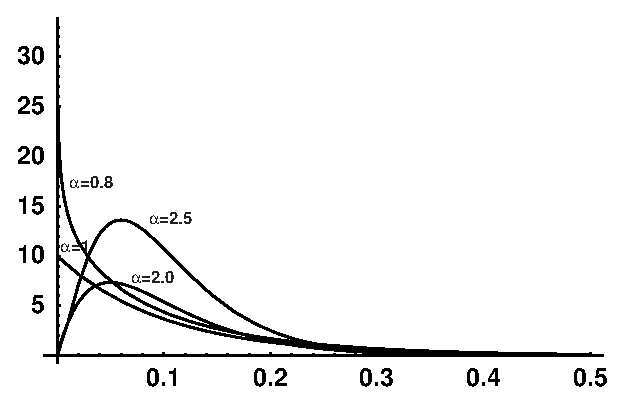
\includegraphics{gamma.eps}}
\end{center}
\caption{Examples of a gamma distribution.}\label{fig:asrv}
\end{figure}

The mean substitution rate in each curve above is 0.1. The curves
differ only in the value of a parameter, $\alpha$, called the ``shape
parameter.'' The shape parameter gives a nice numerical description of
how much rate variation there is, except that it's backwards. The
larger the parameter, the less among-site rate variation
there~is.\index{among-site rate variation!shape parameter}

\section*{The neutral theory of molecular evolution}

I didn't make a big deal of it in what we just went over, but in
deriving the Jukes-Cantor equation I used the phrase ``substitution
rate'' instead of the phrase ``mutation rate.''\footnote{In fact, I
  just mentioned the distinction in passing in two different
  footnotes.} As a preface to what is about to follow, let me explain
the difference.\index{mutation rate}\index{substitution rate}

\begin{itemize}

\item {\it Mutation rate\/} refers to the rate at which changes are
  incorporated into a nucleotide sequence during the process of
  replication, i.e., the probability that an allele differs from the
  copy of that allele in its parent from which it was derived. {\it
    Mutation rate\/} refers to the rate at which mutations
  arise.\index{mutation rate}

\item An allele substitution occurs when a newly arisen allele is
  incorporated into a population, e.g., when a newly arisen allele
  becomes fixed in a population. {\it Substitution rate\/} refers to
  the rate at which allele substitutions occur.\index{substitution rate}

\end{itemize}

\noindent Mutation rates and substitution rates are obviously
related{\dash}substitutions can't happen unless mutations occur, after
all{\dash}, but it's important to remember that they refer to
different processes.

\section*{Early empirical observations}

By the early 1960s amino acid sequences of hemoglobins and cytochrome
{\it c\/} for many mammals had been determined. When the sequences
were compared, investigators began to notice that the number of amino
acid differences between different pairs of mammals seemed to be
roughly proportional to the time since they had diverged from one
another, as inferred from the fossil record. Zuckerkandl and
Pauling~\cite{Zuckerkandl-Pauling65} proposed the {\it molecular clock
hypothesis\/} to explain these results. Specifically, they proposed
that there was a constant rate of amino acid substitution over
time. Sarich and Wilson~\cite{Sarich-Wilson67,Wilson-Sarich69} used
the molecular clock hypothesis to propose that humans and apes
diverged approximately 5 million years ago. While that proposal may
not seem particularly controversial now, it generated enormous
controversy at the time, because at the time many paleoanthropologists
interpreted the evidence to indicate humans diverged from apes as much
as 30 million years ago.\index{molecular clock}

One year after Zuckerkandl and Pauling's paper, Harris~\cite{Harris66}
and Hubby and Lewontin~\cite{Hubby-Lewontin66,Lewontin-Hubby66} showed
that protein electrophoresis could be used to reveal surprising
amounts of genetic variability within populations. Harris studied
10 loci in human populations, found three of them to be polymorphic,
and identified one locus with three alleles. Hubby and Lewontin
studied 18 loci in {\it Drosophila pseudoobscura\/}, found seven to be
polymorphic, and five that had three or more alleles.

Both sets of observations posed real challenges for evolutionary
geneticists. It was difficult to imagine an evolutionary mechanism
that could produce a constant rate of substitution. It was similarly
difficult to imagine that natural selection could maintain so much
polymorphism within populations. The ``cost of selection,'' as
Haldane~\cite{Haldane-1957} called it would simply be too
high.\index{cost of selection}

\section*{Neutral substitutions and neutral variation}

Kimura~\cite{Kimura68} and King and Jukes~\cite{King-Jukes69} proposed
a way to solve both empirical problems. If the vast majority of amino
acid substitutions are selectively neutral,\footnote{Notice that I
  just said that we're going to assume that the vast majority of
  nucleotide {\it substitutions\/} are selectively neutral. This
  doesn't mean that most nucleotide {\it mutations\/} are selectively
  neutral. Indeed, we'll see that most of them are deleterious.} then
substitutions will occur at approximately a constant rate~(assuming
that substitution rates don't vary over time) and it will be easy to
maintain lots of polymorphism within populations because there will be
no cost of selection. I'll develop both of those points in a bit more
detail in just a moment, but let me first be precise about what the
neutral theory of molecular evolution actually proposes. More
specifically, let me first be precise about what it does {\it not\/}
propose. I'll do so specifically in the context of protein evolution
for now, although we'll broaden the scope later.

\begin{itemize}

\item {\it The neutral theory asserts that alternative alleles at
    variable protein loci are selectively neutral.} This does {\it
    not\/} mean that the locus is unimportant, only that the
  alternative alleles found at this locus are selectively
  neutral.\index{neutral alleles}

\begin{itemize}

\item Glucose-phosphate isomerase is an esssential enzyme. It
  catalyzes the first step of glycolysis, the conversion of
  glucose-6-phosphate into fructose-6-phosphate.

\item Natural populations of many, perhaps most, populations of plants
  and animals are polymorphic at this locus, i.e., they have two or
  more alleles with different amino acid sequences.

\item The neutral theory asserts that the alternative alleles are
  essentially equivalent in fitness, in the sense that genetic drift,
  rather than natural selection, dominates the dynamics of frequency
  changes among them.

\end{itemize}

\item By {\it selectively neutral\/} we do {\it not\/} mean that the
  alternative alleles have no effect on physiology or fitness. We mean
  that the selection among different genotypes at this locus is
  sufficiently weak that the pattern of variation is determined by the
  interaction of mutation, drift, mating system, and migration. This
  is roughly equivalent to saying that $N_es < 1$, where $N_e$ is the
  effective population size and $s$ is the selection coefficient on
  alleles at this locus.\index{selective neutrality}

\begin{itemize}

\item Experiments in {\it Colias\/} butterflies, and other organisms
  have shown that different electrophoretic variants of GPI have
  different enzymatic capabilities and different thermal
  stabilities. In some cases, these differences have been related to
  differences in individual performance.

\item If populations of {\it Colias\/} are large and the differences
  in fitness associated with differences in genotype are large, i.e.,
  if $N_es > 1$, then selection plays a predominant role in
  determining patterns of diversity at this locus, i.e., the neutral
  theory of molecular evolution would not apply.

\item If populations of {\it Colias\/} are small or the differences in
  fitness associated with differences in genotype are small, or both,
  then drift plays a predominant role in determining patterns of
  diversity at this locus, i.e., the neutral theory of molecular
  evolution applies.

\end{itemize}

\end{itemize}

\noindent In short, the neutral theory of molecular really asserts
only that observed amino acid substitutions and polymorphisms are {\it
effectively\/} neutral, not that the loci involved are unimportant or
that allelic differences at those loci have no effect on
fitness.\index{neutral theory!effective neutrality}\index{effective neutrality}

\subsection*{The rate of molecular evolution}

We're now going to calculate the rate of molecular evolution, i.e.,
the rate of allelic substitution, under the hypothesis that mutations
are selectively neutral.\footnote{Notice that contrary to what I said
  earlier, here I am assuming that {\it mutations\/} are neutral, not
  just substitutions.} To get that rate we need two things: the rate
at which new mutations occur and the probability with which new
mutations are fixed. In a word equation\index{molecular
  clock!derivation}
\begin{eqnarray*}
\mbox{\# of substitutions/generation} &=& (\mbox{\# of mutations/generation})\times(\mbox{probability
  of fixation}) \\
\lambda &=& \mu_0p_0 \quad .
\end{eqnarray*}
Surprisingly,\footnote{Or perhaps not.} it's pretty easy to calculate
both $\mu_0$ and $p_0$ from first principles.

In a diploid population of size $N$, there are $2N$ gametes. The
probability that any one of them mutates is just the mutation rate,
$\mu$, so
\begin{equation}
\mu_0 = 2N\mu \quad . \label{eq:mu-0}
\end{equation}
To calculate the probability of fixation, we have to say something
about the dynamics of alleles in populations. Let's suppose that we're
dealing with a single population, to keep things simple. Now, you have
to remember a little of what you learned about the properties of
genetic drift. If the current frequency of an allele is $p_0$, what's
the probability that is eventually fixed?  $p_0$. When a new mutation
occurs there's only one copy of it,\footnote{By definition. It's new.}
so the frequency of a newly arisen mutation is $1/2N$ and
\begin{equation}
p_0 = \frac{1}{2N} \quad . \label{eq:p-0}
\end{equation}
Putting~(\ref{eq:mu-0}) and~(\ref{eq:p-0}) together we find
\begin{eqnarray*}
\lambda &=& \mu_0p_0 \\
        &=& (2N\mu)\left(\frac{1}{2N}\right) \\
        &=& \mu \quad .
\end{eqnarray*}
In other words, if mutations are selectively neutral, the substitution
rate is equal to the mutation rate. Since mutation rates are (mostly)
governed by physical factors that remain relatively constant, mutation
rates should remain constant, implying that substitution rates should
remain constant if substitutions are selectively neutral. In short, if
mutations are selectively neutral, we expect a molecular
clock.\index{molecular clock}

\subsection*{Diversity in populations}

Protein-coding genes consist of hundreds or thousands of nucleotides,
each of which could mutate to one of three other
nucleotides.\footnote{Why three when there are four nucleotides?
  Because if the nucleotide at a certain position is an A, for
  example, it can only {\it change\/} to a C, G, or T.} That's not an
infinite number of possibilities, but it's pretty large.\footnote{If a
  protein consists of 400 amino acids, that's 1200 nucleotides. There
  are $4^{1200} \approx 10^{720}$ different sequences that are 1200
  nucleotides long. For context, there are only about
  $3.28 \times 10^{80}$ elementary particles in the
  universe~(\url{https://www.popularmechanics.com/space/a27259/how-many-particles-are-in-the-entire-universe/}).}
It suggests that we could treat every mutation that occurs as if it
were completely new, a mutation that has never been seen before and
will never be seen again. Does that description ring any bells? Does
the infinite alleles model sound familiar? It should, because it
exactly fits the situation I've just
described.\index{mutation!infinite alleles model}

Having remembered that this situation is well described by the
infinite alleles model, I'm sure you'll also remember that we can
calculate the equilibrium inbreeding coefficient for the infinite
alleles model, i.e.,
\[
f = \frac{1}{4N_e\mu + 1} \quad .
\]
What's important about this for our purposes, is that to the extent
that the infinite alleles model is appropriate for molecular data,
then $f$ is the frequency of homozygotes we should see in populations
and $1-f$ is the frequency of heterozygotes. So in large populations
we should find more diversity than in small ones, which is roughly
what we do find. Notice, however, that here we're talking about
heterozygosity at individual nucleotide positions,\footnote{Since the
  mutation rate we're talking about applies to individual nucleotide
  positions.} not heterozygosity of halpotypes.

\section*{Conclusions}

In broad outline then, the neutral theory does a pretty good job of
dealing with at least some types of molecular data. I'm sure that some
of you are already thinking, ``But what about third codon positions
{\it versus\/} first and second?'' or ``What about the observation
that histone loci evolve much more slowly than interferons or MHC
loci?''  Those are good questions, and those are where we're going
next. As we'll see, molecular evolutionists have elaborated the
framework extensively\footnote{That mean's they've made it more
  complicated.} in the last fifty years, but these basic principles
underlie every investigation that's conducted. That's why I wanted to
spend a fair amount of time going over the logic and
consequences. Besides, it's a rare case in population genetics where
the fundamental mathematics that lies behind some important
predictions are easy to understand.\footnote{It's the concepts that
  get tricky, not the algebra, or at least that's what I think.}

\bibliography{popgen}
\bibliographystyle{plain}

\ccLicense

\end{document}


